\chapter{2013 Track \& Field \label{chap:track-field}}

Track \& Field encompasses a wide variety of unicycling disciplines that are done either on a racing track (similar to an athletics track) or in the ``Field''.
It includes all of the disciplines mentioned in this chapter, and all similar ones that are not described in the Rulebook.
Road Racing disciplines (part \ref{part:road_racing}) and Muni disciplines (part \ref{part:muni}) are among the disciplines that have their own parts in this Rulebook, and are not considered to be Track \& Field disciplines.

\section{Track \& Field Categories}

\subsection{Male/Female}
Racing competition is held in two separate divisions: Male and Female.
No heat of any race shall be composed of both male and female riders without the approval of the Racing Referee.

\subsection{Age Groups \label{subsec:track-field_racing-categories_age-groups}}
The following age groups are the minimum required by the IUF to be offered at the time of registration for any Track \& Field discipline: 0-10 (20$"$), 0-13, 14-18, 19-29, 30-UP.
Convention hosts are free to offer more age groups, and often do.
For example, a full range of offered age groups might look like 0-8 (20$"$), 9- 10 (20$"$), 0-12, 13-14, 15-16, 17-18, 19-29, 30-39, 40-49, 50-59, 60-UP.
All age groups must be offered as male and female age group.

\subsection{Wheel Sizes}
Wheel sizes for track racing are 20$"$, 24$"$ and 29$"$.
Additional groups for 16$"$ or other wheels can be added.
Age groups for sizes less than 24$"$ should allow for riders of those ages to also ride 24$"$ wheels with older riders, hence the 0-13 (24$"$) group.
All riders in age groups between 0 and 10 will race a 10m Wheel Walk, and 10m Ultimate Wheel, if used (instead of 30m).

\subsection{Finals}
At Unicons, a `final' must be held for each of the following races: 100m, 400m, 800m, One Foot, and Wheel Walk. 
For any other Track \& Field discipline, a `final' may be held at the discretion of the organizer, after all age group competition for that discipline has been completed.

For disciplines that are run in heats, such as 100m races or relay races, this will take the form of a final heat. 
For disciplines that are not run in heats, such as IUF slalom or slow race, the final will take the form of successive attempts by the finalists.

The riders posting the best results in age group competition are entitled to compete in the final.
They can be called ``finalists''.
The number of finalists will be the same as the number of usable lanes on the track.
The same number of finalists applies for finals that don’t use lanes. 
Finals are composed regardless of age group, but male and female competitors are in separate finals.

Finals are subject to the same rules as age group competition, including false start rules and number of attempts.

The best result in a final determines the male or female Champion for that discipline (World Champion in the case of Unicon).

If a finalist disqualifies, gets a worse result, or doesn’t compete in the final, his/her result in age group competition will still stand.
The male and female winners of the finals will be considered the Champions for those disciplines, even if a different rider posted a better result in age group competition.
Speed records can be set in both age group competition and finals.

In disciplines for which no finals are held, finalist status will still be awarded on the basis of results in age group competition.
Accordingly, riders posting the best results in each discipline are the Champions for that discipline.

\section{Unicycles For Racing}
Only standard unicycles may be used.
Riders may use different unicycles for different racing events, as long as all comply with the rules for events in which they are entered.

\subsection{Wheel Size}
For events divided by wheel size, there is a maximum allowable tire diameter for each category: 
\begin{itemize}
\item For 29$"$ wheels, the outside diameter of the tire may not be larger than 768mm.
\item For 24$"$ wheels, the outside diameter of the tire may not be larger than 618mm.
\item For 20$"$ wheels, the outside diameter of the tire may not be larger than 518mm.
\item For 16$"$ wheels, the outside diameter of the tire may not be larger than 418mm.
\end{itemize}
For any tire in question, its outside diameter must be accurately measured.

\subsection{Crank Arm Length}
Excepting 29$"$ wheels, this is the minimum allowable length, measured from the center of the wheel axle to the center of the pedal axle.
Longer sizes may be used.
\begin{itemize}
\item For 29$"$ wheels, any size crank arms may be used.
\item For 24$"$ wheels, crank arms may be no shorter than 125mm.
\item For 20$"$ wheels, crank arms may be no shorter than 100mm.
\item For 16$"$ wheels, crank arms may be no shorter than 89mm.
\end{itemize}

\subsection{Pedals}
In all track racing events, shoes must not be fixed to the pedals in any way (no click-in pedals, toe clips, tape, magnets or similar).

\section{Safety Gear}
Riders must wear shoes, kneepads and gloves (definitions in chapter \ref{chap:general_definitions}).
For High Jump, Long Jump and unlimited races riders must wear also helmets. The Referee has final say on whether a rider’s safety equipment is sufficient. The Starter will remove from the starting line-up any riders not properly equipped to race, including riders with dangerously loose shoelaces. A Host is allowed to make helmets and/or kneepads mandatory for track races but it must be announced when registration is opened and must appear as a extra point to check for each discipline the competitor registers for.

\section{Starting}
Riders start mounted, holding onto a starting post or other support.
Unicycle riders need to be leaning forward before the starting gun fires, so the Starter will give a four-count start.
Example: ``One, two, three, BANG!''
This allows riders to predict the timing of the gun, for a fair start.
There should be about 3/4 second between each element in the count, with the same amount of time between each of them.
Starters should practice this before the races begin.
Timing of the count is very important for an accurate start.
This count can be in the local language, or a language agreed upon before competition starts.

As an alternative a Startbeep apparatus can be used.
In that case we have a six-count start.
Example: ``beep - beep -beep - beep - beep - buup!''
The interbeep timing is one second.
The first 5 beeps have all the same frequency.
The final tone (buup) has a slightly higher frequency, so that the racer can easily distinguish this tone from the rest.

Riders start with the fronts of their tires (forward most part of wheel) behind the edge of the starting line that is farthest from the finish line.
Rolling starts are not permitted in any race.
However, riders may start from behind the starting line if they wish, provided all other starting rules are followed.
Riders may lean before the gun fires, but their wheels may not move forward at any time.
Rolling back is allowed, but nothing forward.
Riders may place starting posts in the location most comfortable for them, as long as it doesn't interfere with other riders.

\subsection{Riders Must Be Ready}
Riders must be ready when called for their races.
Riders not at the start line when their race begins may lose their chance to participate.
The Starter will decide when to stop waiting, remembering to consider language barriers, and the fact that some riders may be slow because they are helping run the convention.

\section{False Starts}
A false start occurs if a rider's wheel moves forward before the start signal, or if one or more riders are forced to dismount due to interference from another rider or other source.

There are two options on how to deal with false starts:
\begin{itemize}
\item \textbf{One False Start Allowed Per Rider:}
In case of a false start, the heat is restarted.
Any rider(s) who caused their personal first false start may start again.
Any rider(s) causing their personal second false start are disqualified.
\item \textbf{One False Start Allowed Per Heat:} 
In case of a false start, the heat is restarted.
For the first false start of a particular heat, all riders may start again.
Thereafter, any rider(s) causing a false start are disqualified.
This option should not be used without an electronic false start monitoring system.
\end{itemize}
If a heat has to be restarted, the Starter will immediately recall the riders, for example by firing a gun or blowing a whistle or other clear and pre-defined signal.
It is only the earliest false starting rider who gets assigned this false start and might get disqualified.

\section{Finishes \label{sec:track-field_finishes}}
These are determined by the front of the tire crossing over the edge of the finish line that is nearest to the starting line.
Riders are timed by their wheels, not by outstretched bodies.
Riders must cross the line mounted and in control of the unicycle.
``Control'' is defined by the rearmost part of the wheel crossing completely over the finish line with the rider having: 
\begin{enumerate}
\item[(a)] Both feet on the pedals in normal races; or 
\item[(b)] One foot on a pedal in one foot races; or 
\item[(c)] At least one foot on the wheel in wheel walk races.
\end{enumerate}
In races where dismounting is allowed (800m, Relay, etc.), in the event of a dismount at the finish line the rider must back up, remount and ride across the finish line again.
In races where dismounting is not allowed, the rider is disqualified.

\subsection{Judging Finish Line Dismounts}
One or more officials are required at the finish line to judge dismounts in all races where dismounting is allowed.
These officials must be appointed by the racing referee so they fully understand their crucial job.
The finish line judges are the voice of authority on whether riders must remount and cross the finish line again.
Any riders affected must be clearly and immediately signaled to return to a spot before the finish line, remount without overlapping the finish line, then ride across it again.
The path for backing up may involve going around any finish line timing or optical equipment to prevent data problems for other riders in the race.

\subsection{Timing Penalty For Finish Line Dismounts}
In electronically timed races, it's possible that no time will be recorded for the rider's successful finish.
Instead of recording an actual finish time, the rider's time will be recorded as 0.01 seconds faster than the next rider to cross the line after their remount and crossing.
If the rider in question is the last one on the track, the time recorded should be their actual time crossing the finish line after their remount.

After the rider has successfully finished the race and there is no correct time for that rider, the rider's finishing time will be calculated based on the time of the next rider to cross the finish line after the rider in question properly finished.
The rider will receive a time penalty which will make his or her time 0.01 second faster than the rider who came after their successful finish.

\section{Lane Use}
In most races, a rider must stay in his or her own lane, except when the rider has to swerve to avoid being involved in a crash.
In this case the rider can decide to have a second try.
Otherwise a rider who goes outside their lane is disqualified immediately.
Going outside a track lane means that the tire of the unicycle touches the lane of another rider.
Riding on the marking is allowed.
No physical contact between riders is allowed during racing.
200m and 400m races are started with a stagger start.
The 800m race may be started in one of two ways:
\begin{itemize}
\item \textbf{Waterfall Start:} This is a curved starting line that places all riders an equal distance from the first turn.
If a waterfall start is used, non-lane rules apply (see below).
\item \textbf{Stagger Start:} Riders are started in separate lanes, at separate locations.
They must stay in their lanes for a specified distance before they may `cut in' to the inside lanes.
Lane rules apply only up to this point.
\end{itemize}

\subsection{Non-Lane Races \label{subsec:track-field_lane-use_non-lane-races}}
This applies to 800m and other events without lanes.
No physical contact between riders is allowed.
Riders must maintain a minimum of one (24$"$) wheel diameter (618mm as judged by eye) between each other when passing, and at all other times.
This is measured from wheel to wheel, so that one rider passing another may come quite close, as long as their wheels remain at least 618mm apart.

\section{Lane Assignments}
At some conventions, lanes are pre-assigned at time of registration.
At other conventions, riders decide among themselves.
If riders disagree, the Clerk makes lane assignments.
In races where more than one heat is necessary per age group, every effort must be made to see that the fastest riders compete in the same heat.
If the track has undesirable lanes due to potholes or other problems, this should be considered when lanes are assigned.
A very bad or dangerous lane might not be used at all.
The Referee can override the Clerk's choice of lane assignments.
The general rule is that riders decide for themselves.

\section{Mixing Age Groups In Heats}
There will be no mixing of age groups, or sexes, in heats except with permission from the Racing Referee.

\section{Passing}
In track races, an overtaking rider must pass on the outside, unless there is enough room to safely pass on the inside.
Riders passing on the inside are responsible for any fouls that may take place as a result.
The passing rider's wheel must remain at least one wheel diameter (618mm) from the slower rider's wheel at all times.
The slower rider must maintain a reasonably straight course, and not interfere with the faster rider.

\section{Dismounting}
A dismount is any time a rider's foot or other body part touches the ground and the unicycle must be remounted.
Except for the 800m, Relay, and some other non-traditional or off-track events, if a rider dismounts, he or she is disqualified.
In races where riders are allowed to remount and continue, riders must immediately remount at the point where the unicycle comes to rest, without running.
If a dismount puts the rider past the finish line, the rider must back up and ride across the line again.
If a rider is forced to dismount due to the actions of another rider, or outside interference, the Referee decides if he or she can enter that race again in another heat.
In non-lane races, if a rider is forced to dismount due to a fall by the rider immediately in front, it is considered part of the race and both riders must remount and continue.
The Referee can override this rule if intentional interference is observed.

\section{Assisting Racers}
In races where riders are allowed to remount, the riders must mount the unicycle completely unassisted.
Spectators or helpers may help the rider to his or her feet and/or retrieve the dropped unicycle, but the rider (and the unicycle) may not have any physical contact with any outside object or person, including a starting block under the wheel, when mounting.

\section{Illegal Riding}
This includes intentionally interfering in any way with another rider, deliberately crossing in front of another rider to prevent him or her from moving on, deliberately blocking another rider from passing, or distracting another rider with the intention of causing a dismount.
A rider who is forced to dismount due to interference by another rider may file a protest immediately at the end of the race.
Riders who intentionally interfere with other riders may receive from the Referee a warning, a loss of placement (given the next lower finishing place), disqualification from that race/event, or suspension from all races.

\section{Protests}
The official protest form must be available to riders at all times.
All protests against racing results must be submitted in writing on the proper form after a race, until 30 minutes after the results are posted.
It is highly recommended that for larger events (like Unicon) this period be extended to 60 minutes.
The form must be filled in completely.
This time may be extended for riders who have to be in other races during that time period.
All protests will be handled within 30 minutes from the time they are received.
Mistakes in paperwork, inaccuracies in placing, and interference from other riders or other sources are all grounds for protests.
All Referee decisions are final, and cannot be protested.

\section{Optional Race-End Cut-Off Time}
It may be necessary to have a maximum time limit for long races, to keep events on schedule.
When this is planned in advance, it must be advertised as early as possible, so attending riders will know of the limit.
Additionally, at the discretion of the Racing Director, a race cut-off time may be set on the day of or during an event.
The purpose of this is to allow things to move on if all but a few slow racers are still on the course.
These cut-offs need not be announced in advance.
At the cut-off time, any racers who have not finished will be listed as incomplete (no time recorded, or same cut-off time recorded for all).
Optionally, if there is no more than one person on the course per age category and awards are at stake, they can be given the following place in the finishing order.
But if each participating age category has had finishers for all available awards (no awards at stake), there is no need to wait.

\section{Minimum Racing Events \label{sec:track-field_minimum-racing-events}}
The following races: 100m, 400m, 800m, One Foot, Wheel Walk, and IUF Slalom, are to be part of every Unicon.
Convention hosts are free to add more racing events.

\section{Track Combined Competition}
The best finishers combined from the 6 racing events listed above will win this title.
Points are assigned for placement in each of the above races, based upon best times in the final heats or finishing age group times in the IUF Slalom.
1st place gets 8, 2nd place 5, 3rd place 3, 4th place 2, and 5th place 1.
Highest total points score is the World Champion; one each for male and female.
If there is a tie, the rider with the most first places wins.
If this still results in a tie, the title goes to the better finisher in the 100m race.
Points are not earned in age group heats.

\section{Traditional Specialty Races}
These races should be part of every Unicon:

\subsection{One Foot}
Riders may pedal with both feet for the first 5 meters, but must be pedaling with only one foot after crossing the 5m line.
The 5m line is judged by looking at the tire contact point.
This means that the foot must have left the pedal when the unicycle tire is touching the 5m line on the track.
The non-pedaling foot may or may not be braced against the unicycle fork.

\subsection{Wheel Walk}
Riders start mounted, with their feet on the tire, and propel the unicycle only by pushing the tire with their feet.
No contact with pedals or crank arms is allowed.
No crank arm restrictions.

\subsection{IUF Slalom}
\begin{figure}[h]
\begin{center}
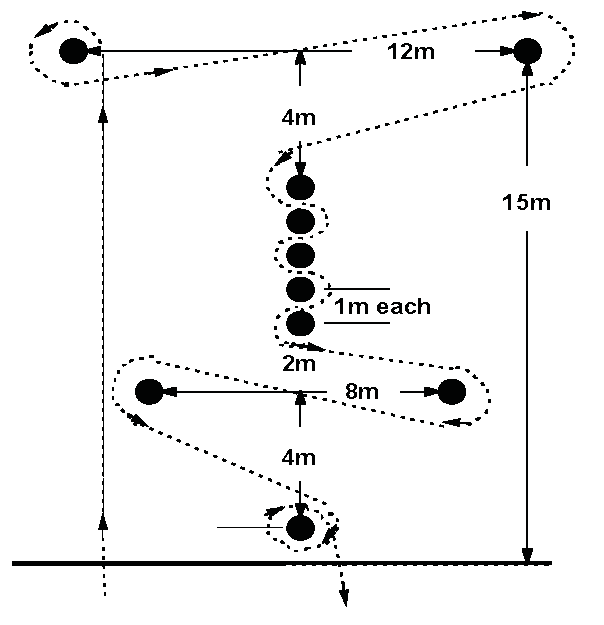
\includegraphics{iuf_slalom}
\end{center}
\vspace{-20pt}
\caption{IUF Slalom Course \label{fig:iuf_slalom}}
\vspace{-10pt}
\end{figure}
Pitured here is the IUF Slalom, in which you must ride around 10 cones in the correct pattern.
Arrows marked on the ground should indicate the direction of the turns for riders unfamiliar with the course.
The rider has to start directly behind the Start line.
The Starter gives the opening, and then the competitor has to start during the next 3 seconds.
The timer is started when any defined point of the tire (for example the part that crosses a low light beam) crosses the start line, and stops when a similar point of the tire crosses the finish line.
If the rider has not yet started after 3 seconds, the timer will start counting anyway.
The rider is not disqualified for this.
Time measurement at start and finish line must be identical to insure accurate time measurement.
It must be secured that riders do not gain momentum before crossing the start line (no flying starts).
Remounting is not allowed. 
Cones may be hit, but not knocked over.
The course must be followed correctly, including the direction of turns.
The last cone must be completely circled before the rider's time is taken at the finish line.
Riders who go the wrong way around a cone can go back and make the turn the correct way with the clock still running.
The cones used are plastic traffic cones.
For official competition, cones must be between 45 and 60cm tall, with bases no more than 30cm square.
The course must be set up accurately.
The proper positions of the cones should be marked on the ground for a cone to be replaced quickly after it has been knocked over.
Riders get two attempts.

\section{Jumping Events \label{sec:track-field_jumping-events}}
Unicycling versions of the High Jump and Long Jump 
\subsection{High Jump}
The rider and unicycle jump over a bar, without knocking it down, and ride away without a dismount.
There are three parts to a successful jump: 
\begin{enumerate}
\item Riders must mount before the start line, to show they are on the unicycle and in control.
The attempt starts when the rider crosses the start line.
The rider may break off from a jumping attempt before leaving the ground, but must then start again from behind the start line.
That attempt then doesn't count.
\item Riders must jump over the bar without knocking the bar off the apparatus.
The bar can be hit as long as it does not fall.
If the bar falls before the rider crosses the finish line, it counts as an unsuccessful attempt.
\item After landing, the rider must stay in control of the unicycle until he cross the finish line without dismounting, touching a hand to the ground or any other object, or knocking down the bar or any of the high jump apparatus.
Riders get two attempts at each height.
The rider starts at a low height and after each successful attempt, the height increases at set intervals until the rider fails to be successful on both attempts.
When the rider fails both attempts, the maximum height that was completed is recorded.
\end{enumerate}

\subsubsection{Unicycles}
Standard unicycles must be used (see definition in chapter \ref{chap:general_definitions}).
No restriction on wheel or crank size.
Metal pedals are allowed for their strength and better grip.
This may make it impossible to hold this event on a sensitive track surface.

\subsubsection{Setup}
Around the High Jump apparatus a circle with a radius of 3 meters must be marked.
This circle is start and finish line.
The rider can cross it wherever he wants.
Riders must ride or hop across the finish line for the attempt to count.
Successfully crossing the finish line is judged the same as in racing (see section \ref{sec:track-field_finishes}).
The bar must be held loosely in the jumping apparatus so it can fall or break away if the rider does not complete the desired height.
Magnetic systems are not allowed.
The bar shall have a minimum diameter of 2cm.

\subsubsection{Broken Unicycle}
If the unicycle breaks during an attempt, a new attempt must be given to the rider.

\subsection{Long Jump}
The rider jumps as far as possible from a jump marker, to a landing without a dismount.
The rider must then continue riding across a finish line to show control.
Riders must clear 3 markers (jump marker, landing marker and finish line) to make the jump count.
Riders may jump with the wheel going forward or sideways.
After landing, the rider must stay in control of the unicycle for the remainder of a 5-meter distance from the jump marker without dismounting, or touching a hand to the ground or any other object.
If the tire touches the jump marker before takeoff or the landing marker, it counts as a foul.
Riders may break off in a run as long as he is between start line and jump marker but if they cross or touch the jump marker, the attempt counts, including fouls.
Riders get two attempts for each length.
The farthest non-fouling, successful jump is recorded.

To avoid endless competitions, the length to jump will always increase by 5cm for each round.
Once there are only 5 riders left, it's up to the riders to decide in which steps they continue.
For each age group the minimum length should be adjusted to a useful level such as 150cm for 15+ and 70cm for 0-15.
The host can adjust this depending on the level at his competition.

\subsubsection{Unicycles}
Standard unicycles must be used (see definition in chapter \ref{chap:general_definitions}).
No restriction on wheel or crank size.
Metal pedals are allowed for their strength and better grip.
This may make it impossible to hold this event on a sensitive track surface.

\subsubsection{Setup}
The riding area consists of a start line, a jump marker, a landing marker and a finish line 6 meters beyond the jump marker.
Riders must ride or hop across the finish line for the attempt to count.
Successfully crossing the finish line is judged the same as in racing (see section \ref{sec:track-field_finishes}).
The start line must be in the minimum 15 meters in front of the jump marker to be able to accelerate; behind the finish line must be an area which is 7 meter long and 2 meter wide in the minimum as safety zone.
Riders may use all or part of the 15 meters between start line and jump marker.
They are also allowed to start from beside to be able to do accelerated side jumps.
Markers for takeoff and landing (jump marker and landing marker) should be similar in shape to a meter stick, and be at least one meter in width (across the runway), no more than 5mm in height (above the runway), and no less than 3 centimeters in depth (front to back).
A Long Jump competition needs a minimum area of 28x2 meters.

\subsubsection{Judging}
The rider must clear the jump marker and the landing marker without touching them; he also has to clear the finish line to make it a valid jump.
Jump distance is measured between the outer edges of the jump and landing marker.
There has to be at least one judge (better two) to look at the markers.
For national championships and Unicons, two judges are always needed; one to observe each marker.

\subsubsection{Broken Unicycle}
If the unicycle breaks during the jump or landing, the rider will be given a new attempt.

\section{Alternate, Optional or Fun Events \label{sec:track-field_alternate-optional-fun-events}}
These are optional events, not guaranteed to be included in every unicycle convention.
They can be held with as much, or as little, level of formality and importance the host chooses.
Age group breakdown is also up to the host.
All of the events in this section have been run before, using these rules.
If a large convention advertises events with the names of the ones detailed in this section, they must use the rules provided here.
If hosts desire to do variations on these rules, the events must be labeled accordingly.
Example: ``Track Gliding; Modified''.
In cases such as this, hosts must remember to provide detailed rules for these events at the same time the events are announced.

\subsection{Relay (Track)}
Usually 4 x 100m or 4 x 400m like in athletics.

The takeover zones are 20m long and must be marked on the track.
Riders may remount if necessary, and must pick up the baton if it is dropped.
The handover of the baton must be within the takeover zone.
This means that before the baton crosses the start mark of the takeover zone \textit{only} the incoming rider is in touch with the baton and at the end of the takeover zone \textit{only} the outgoing rider is in touch with the baton.
Riders may not throw the baton to make a pass and may not touch the ground with any part of their body while making a pass.
If the baton is not handed over within the marked takeover zone, the team will be disqualified.
Leaving of the lane within the takeover zone or when remounting does not result in disqualification as long as the riders do not obstruct, impede or interfere with another rider's progress.
There is no defined preparation area for the next riders as long as they stay within their lanes.

Mixed male/female teams may be used, and reasonable age groups may be used depending on the number of expected competitors of the event.
Each relay team may have any mix of ages, the age of the oldest rider determines the age group.

\subsection{Coasting Events}
An event to determine which rider coasts the furthest distance.
Riders' coasting distances are measured from a `starting line' with a 5 meter minimum, which will be marked by a `qualifying line.'
If the rider does not cross the qualifying line it will count as a failed attempt.
The farthest distance from the line wins.
The distance is measured to the rearmost part of the rider that touches the ground when dismounting, or to the rear of the tire where the rider stops coasting.
Remounting is not allowed.
Riders must not touch any part of their tires, wheels or pedals while coasting.
Riders get two attempts.
If a rider crosses the coasting line (front of the tire) not in coasting position, he or she is disqualified in that attempt.
The riding surface should be as smooth and clean as possible, and it may be straight or curved.
Ample time must be allowed for all competitors to make some practice runs on the course before the official start.
The type of event(s) to be used should be announced well in advance of the competition.
Crank arm rules do not apply in any coasting or gliding events.

\subsubsection{Road Coasting}
This event is best held on a roadway with a very slight downward slope.
Riders are allowed an unlimited distance to speed up and start coasting before the starting line.

\subsubsection{Track Coasting \label{subsubsec:track-field_alternate-optional-fun-events_coasting_track-coasting}}
30 meter speed-up distance.
This event is held only on a track, or a very level, smooth surface.
Wind must be at a minimum for records to be set and broken.
This event can be compared with other races at different tracks worldwide.

\subsubsection{Downhill Coasting}
This is a speed coasting event.
Riders start from a standstill, or speed up to the `starting line'.
Riders are timed over a measured distance to the finish line.
Dismounts before the finish line disqualify the rider in that attempt.
The slope must be very gradual for this event to be safe, and helmets are mandatory.

\subsubsection{Indoor Coasting}
30 meter starting distance.
This event is held indoors in a gym, or on a very level, smooth surface.
Rider will coast in a circle on the outer edge of the gym, separated by cones.
Both directions are allowed for the start (clockwise or counterclockwise), and rider will have a maximum of 30m before beginning to coast.
Indoor coasting is the recommended coasting competition at a Unicon.

\subsection{Gliding Events}
Gliding is like coasting, but with one or both feet dragging on top of the tire to provide balance from the braking action.
These events are similar to the coasting events above, with riders gliding for time or distance from a given point.
The rules are the same as for the coasting events (above) with the addition that the riding surface must be dry.
Coasting is allowed.

\subsubsection{Slope Glide Or Track Glide}
A slope glide can be done on a small hill.
Riders start on the hill, gliding down to level ground and continuing as far as they can before stopping.
This event can have a limited starting distance, or no starting distance at all, with riders gliding from a dead stop.
If it is a Track Glide, it is held on a track with the same rules as Track Coasting (see section \ref{subsubsec:track-field_alternate-optional-fun-events_coasting_track-coasting}).

\subsubsection{Downhill Glide}
A downhill race for speed.
Riders start from a standstill, or speed up to the `starting line.'
Riders are timed over a measured distance to the finish line.
Dismounts before the finish line disqualify the rider in that attempt.
Helmets are mandatory.

\subsection{Slow Forward}
The object is to ride in a continuously forward motion as slowly as possible without stopping, going backward, hopping, or twisting more than 45 degrees to either side.
Two different board sizes are used: Age 0-10: 10m x 30cm.
Age 11-UP: 10m x 15cm.
The Slow Race is measured using the bottom of the unicycle wheel.
Riders start with the bottom of the wheel on the starting line.
On command by the Starter, the rider must immediately start forward motion and let go of starting posts.
The timer stops the watch when the bottom of the tire touches either the finish line, or the ground after the line on boards that end at the finish line.
Riders can be disqualified for very slight stops or backward motions, twisting more than 45º to the side, riding off the sides of the board, or dismounting.
Riders get two attempts.
There are no crank arm length or wheel size restrictions for this event.
No safety gear is required.

\subsection{Slow Backward}
This is the same as the slow forward race \textit{except}: 0-10 ride on 60cm board, 11-Up ride on 30cm board.

\subsection{700c Racing}
Races of any length and type can also be conducted in a 700c wheel category.
\begin{itemize}
\item Maximum wheel diameter: 768mm.
\item If these races are intended to exclude 24$"$ wheels, sizes must be greater than 618mm.
\item No restrictions on crank length.
\item Beyond these, 700c unicycles must comply with all other requirements for racing unicycles.
\item The host may choose age groups.
\end{itemize}

\subsection{Unlimited Track Racing}
An unlimited race is one in which there are no unicycle size restrictions.
Any size wheels, any length crank arms, giraffes or any types of unicycles (see definition in chapter \ref{chap:general_definitions}) are allowed.
All other Track racing rules apply.

\subsection{Juggling Unicycle Race}
The traditional distance is 50m.
Riders use the 5m line from the One-Foot Race, and must be juggling when they cross this line.
Three or more non-bouncing objects must be used.
If an object is dropped (hits the ground) or the juggling pattern is otherwise stopped, the rider is disqualified.
Two balls stopping in one hand during a 3-ball cascade is defined as stopping.
Riders who start by juggling four or more objects may drop one, as long as their pattern continues, unbroken, into three.
The juggling pattern must be `in control' when the rider crosses the finish line.
`Control' is determined by the Referee.

\subsection{Ultimate Wheel Race}
An ultimate wheel is a unicycle with no frame or seat.
The traditional distance is 10m for 0-10 riders, and 30m for 11-UP riders.
Maximum wheel size is 618mm (24$"$) for all ages, with 125mm minimum crank arm length or 250mm between pedal holes.
The host may allow other limitations, or none, if these details are announced well in advance.

\subsection{50m Fast Backward}
Riders must face and pedal backward.
The Starter lines up the rear of the tire above the start line.
Helmets are mandatory.
Timing is stopped when the rear of the tire crosses the finish line.

\subsection{Medley}
This is a race involving riding several different ways of riding.

\textbf{Example:} Forward 25m, seat in front 25m, one foot 25m, hopping 10m, with 5m transition areas.
Rules are set by the host.
Remounting is allowed.

\subsection{Slow Giraffe Race}
This is the same as slow forward, but on giraffes.
Helping hands can be used as starting posts.
No limits on size or gear ratio, but unicycles must have their pedal axle above the wheel axle, with a chain, belt, or other form of drive system.